\label{chapter:resultados}

O presente capítulo consiste em apresentar o planejamento, execução, e  análise dos resultados referente ao método proposto. Assim,  visando avaliar de forma experimental o sistema computacional desenvolvido a partir do método proposto, denominado de INEXT, para identificação e localização de objeto em edifícios utilizando RFID.

\section{Planejamento e projeto dos experimentos}

Esta avaliação experimental consiste em avaliar o INEXT, tendo como questões principais a identificação e localização de objetos em ambientes confinados e então o gerenciamento dos objetos. Em virtude disso, foi definida as seguintes questões:

\begin{itemize}

    \item[QP1]: O sistema INEXT consegue identificar e rastrear os objetos em um âmbito confinado?
    \item[QP2]: Quais vantagens o sistema INEXT prove em relação ao gerenciamento dos objetos em edifícios?
    \item[QP3]: O sistema INEXT é capaz de gerar de forma automática o inventário de objetos em um âmbito confinado?
    
\end{itemize}

\par 
Objetivando responder tais questões de pesquisa, foram utilizados um Arduíno Nano V$3.0$ ATmega168 e um computador comunicando-se através da porta serial para simular a segunda sala, pois não disponhamos de duas placas NodeMcu para a comunicação sem fio. Um script na linguagem Python v$3.7.1$ foi adotado para ler os dados da porta serial, criar um objeto JSON e enviar para o servidor, tais códigos estão disponíveis no repositório deste trabalho (endereço mencionado no \autoref{chapter:metodo}) dentro da pasta \texttt{prototype\_arduino}. O computador utilizado possui $4$GB de memória RAM, processador Intel Core i$5-2500$, HD de $500$GB e sistema operacional Windows $7$ Professional de $64$Bits. 

Os protótipos dos dispositivos de porta podem ser visualizados nas \autoref{fig:prototipo_arduino} e \autoref{fig:prototipo_nodemcu}. A \autoref{fig:prototipo_arduino} mostra o Arduíno Nano juntamente com o leitor RFID RC522 conectados através de \textit{jumpers}, já na \autoref{fig:prototipo_nodemcu} mostra o NodeMcu conectado com o leitor RFID RC522. A prototipação do Arduíno segue abaixo:

\begin{itemize}
    \item $3.3$V - conectado ao pino de $3.3$v no Arduíno, essa conexão faz a alimentação do leitor RFID;
    \item RST (\textit{Reset})- conectado ao pino $9$ do Arduíno;
    \item GND (\textit{graduated neutral density filter}) - conectado ao pino GND do Arduíno;
    \item NC/IRQ (\textit{Interrupt Request})- não utilizado;
    \item MISO (\textit{Master In Slave Out}) - conectado ao pino $12$;
    \item MOSI  (\textit{Master Out Slave In}) - conectado ao pino $11$;
    \item SCK  (\textit{Serial Clock}) - conectado ao pino $13$; e 
    \item SDA/ SS (\textit{Serial Data Line/ Select Slave}) - conectado ao pino $10$.
\end{itemize}    

\begin{comment}
\begin{figure}[H]
              \caption{\label{fig:esq_conexoes_arduino}{Esquema de Conexões Arduíno Nano}}
              \centering
              \includegraphics[width=1\textwidth]{Figuras/esquema_de_conexoes1.PNG}
              \legend{Fonte: Própria}
\end{figure}
\end{comment}

\begin{figure}[H]
              \caption{\label{fig:prototipo_arduino}{Protótipo Arduíno Nano}}
              \centering
              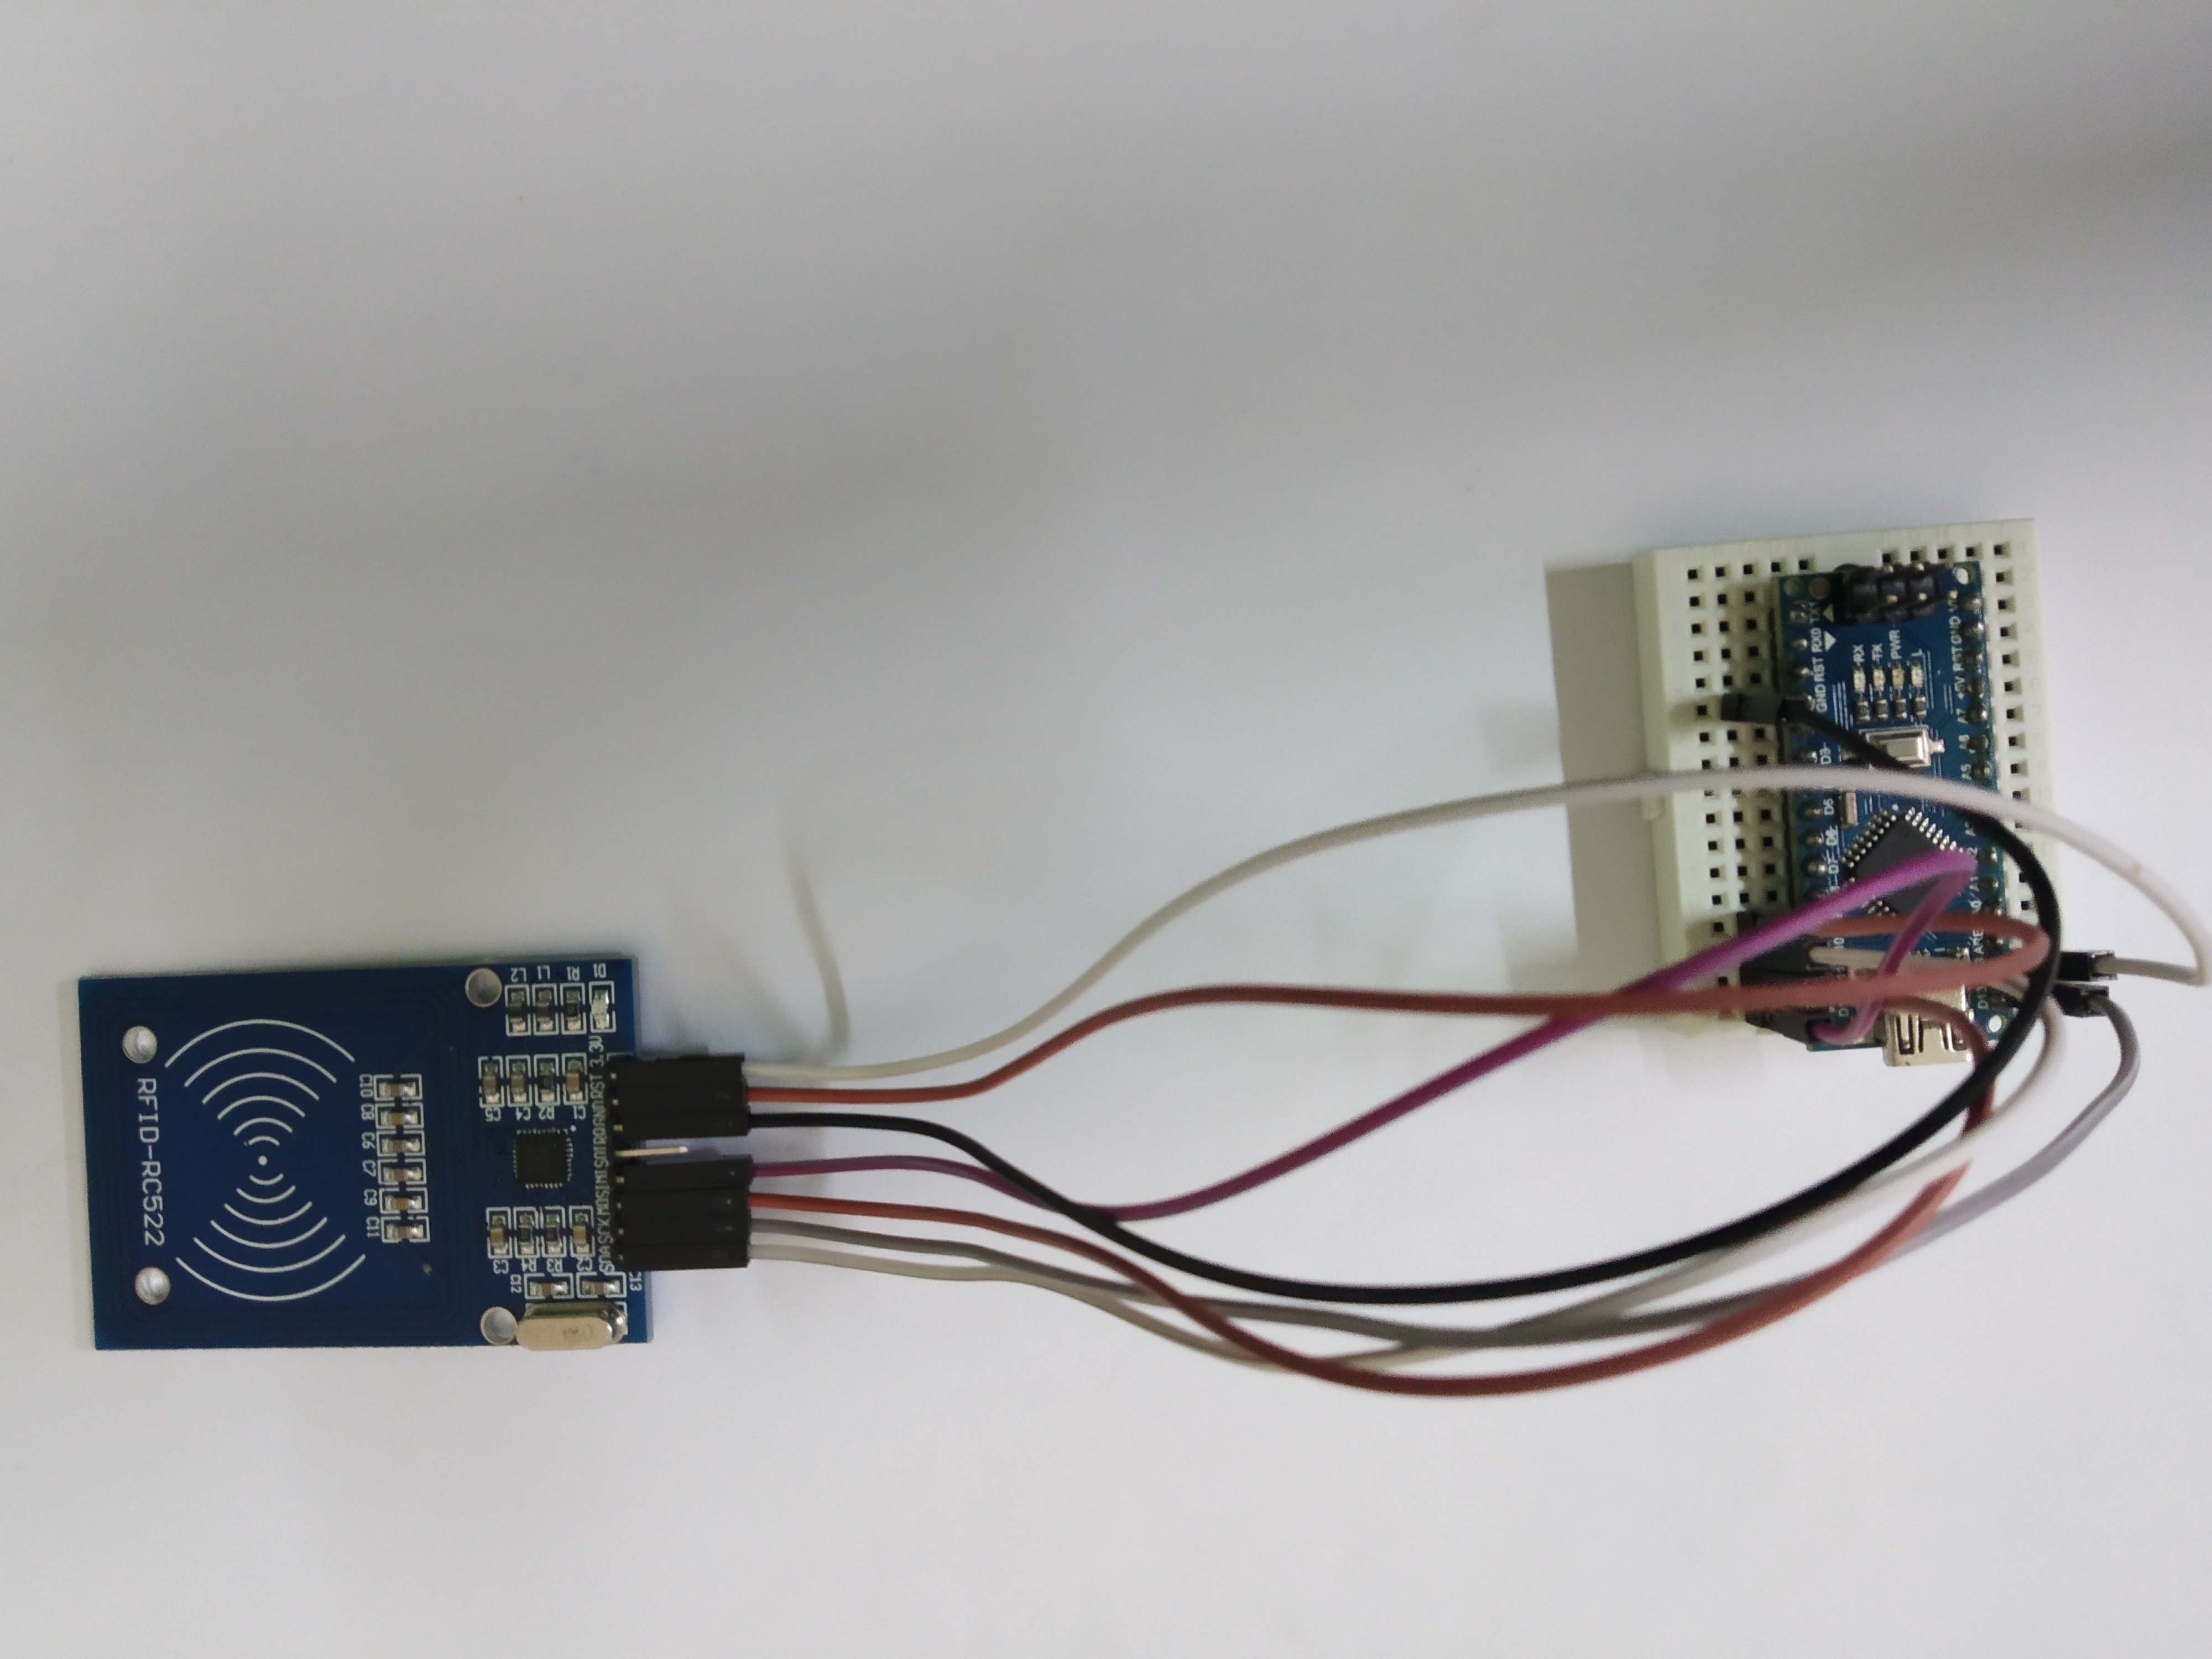
\includegraphics[width=0.7\textwidth]{Figuras/prototype_arduino.png}            \legend{Fonte: Própria}
\end{figure}\begin{figure}[H]
              \caption{\label{fig:prototipo_nodemcu}{Protótipo NodeMcu}}
              \centering
              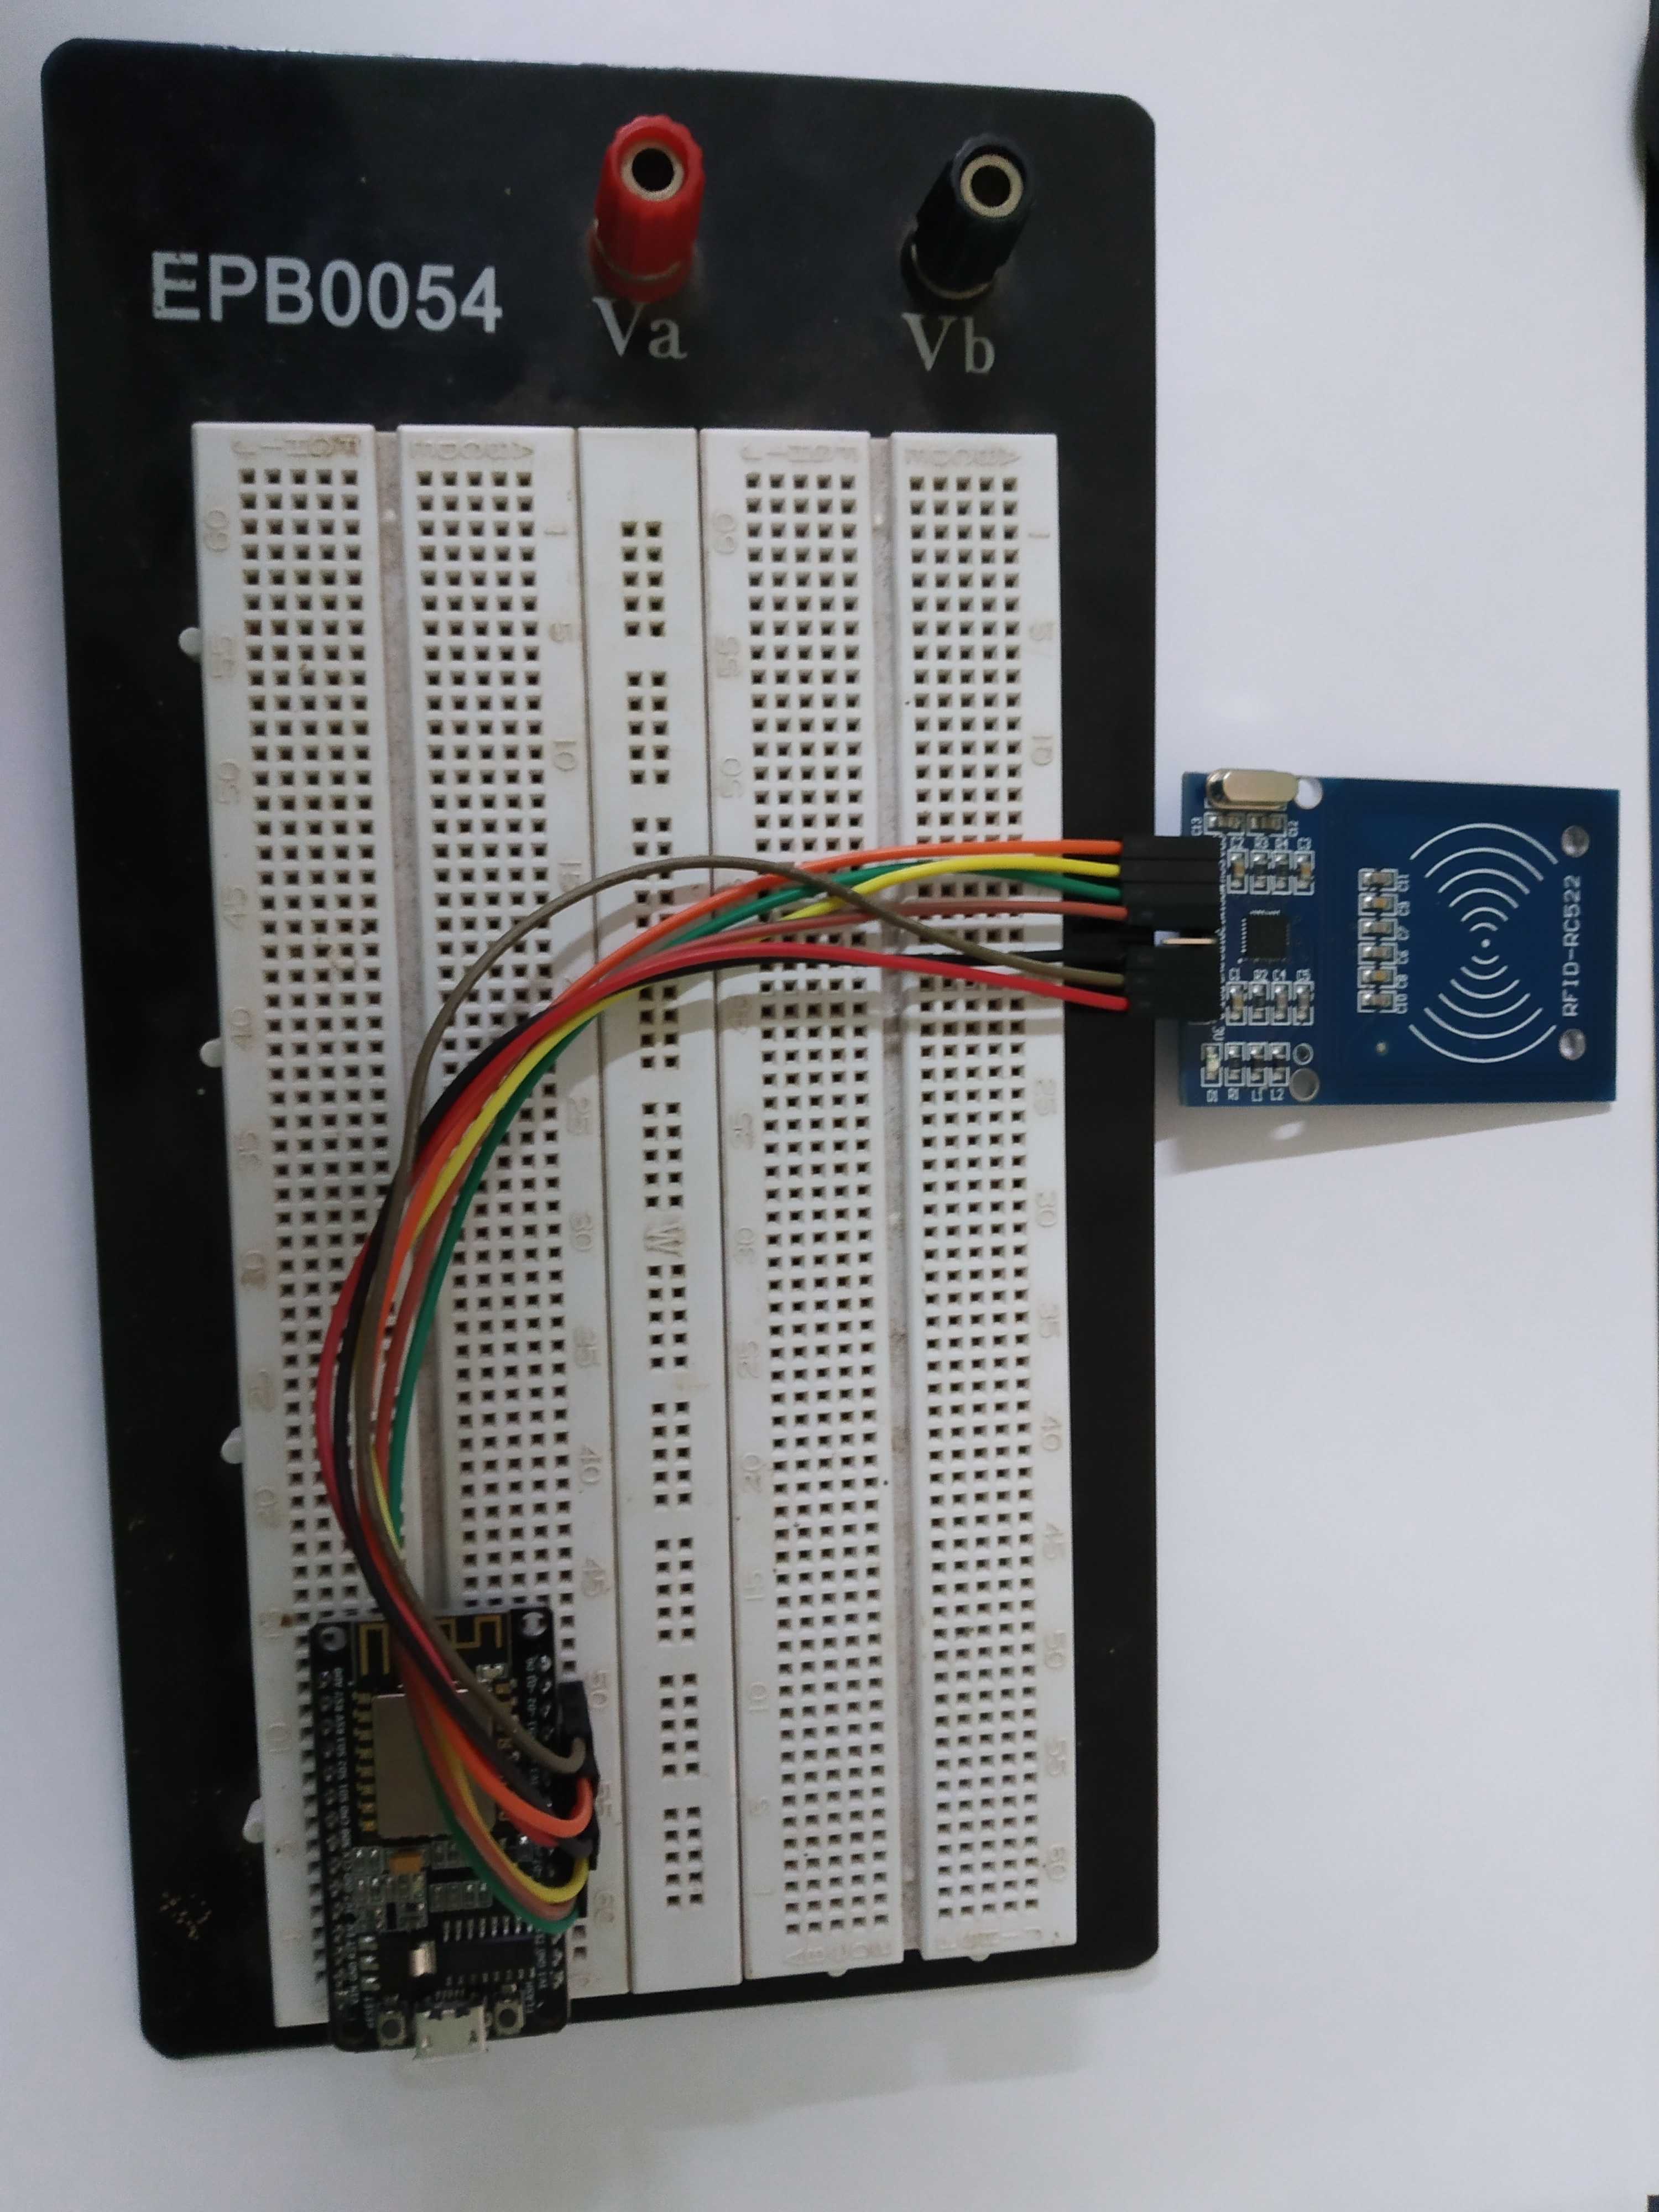
\includegraphics[width=0.5\textwidth]{Figuras/prototype_nodemcu.png}
              \legend{Fonte: Própria}
\end{figure}


\par
Para a simulação do servidor, foi utilizado um notebook com $6$GB de memória RAM, processador Intel Core i$5-4200$, HD de $750$GB, placa de video GeForce $720$M de $2$GB de memória dedicada e sistema operacional Windows $10$ \textit{Home Single Language}. A rede LAN utilizada foi criada através de um roteador TP-LINK modelo TL-WR$720$N. Também foram utilizadas quatro etiquetas RFID passivas, cada uma dessas etiquetas representa um objeto diferente para a simulação.


\par
A execução do experimento aconteceu no cenário apresentado na \autoref{fig:cenario}, foi simulado duas salas e quatro objetos rastreáveis em um edifício. Visando responder as questões foram executados os seguintes testes: 
\textbf{(1)} localização e identificação dos objetos em ambientes confinados, no intuído de obter respostas para a primeira questão de pesquisa; 
\textbf{(2)} criação de restrição de movimentação sobre objetos, afim de verificar se as notificações ao violar restrição são uma forma de se ter melhor gerenciamento dos objetos; e 
\textbf{(3)} levantamento de todos os objetos em todos os ambientes monitorados pelo sistema INEXT.

\begin{figure}[H]
              \caption{\label{fig:cenario}{Cenário de simulação}}
              \centering
              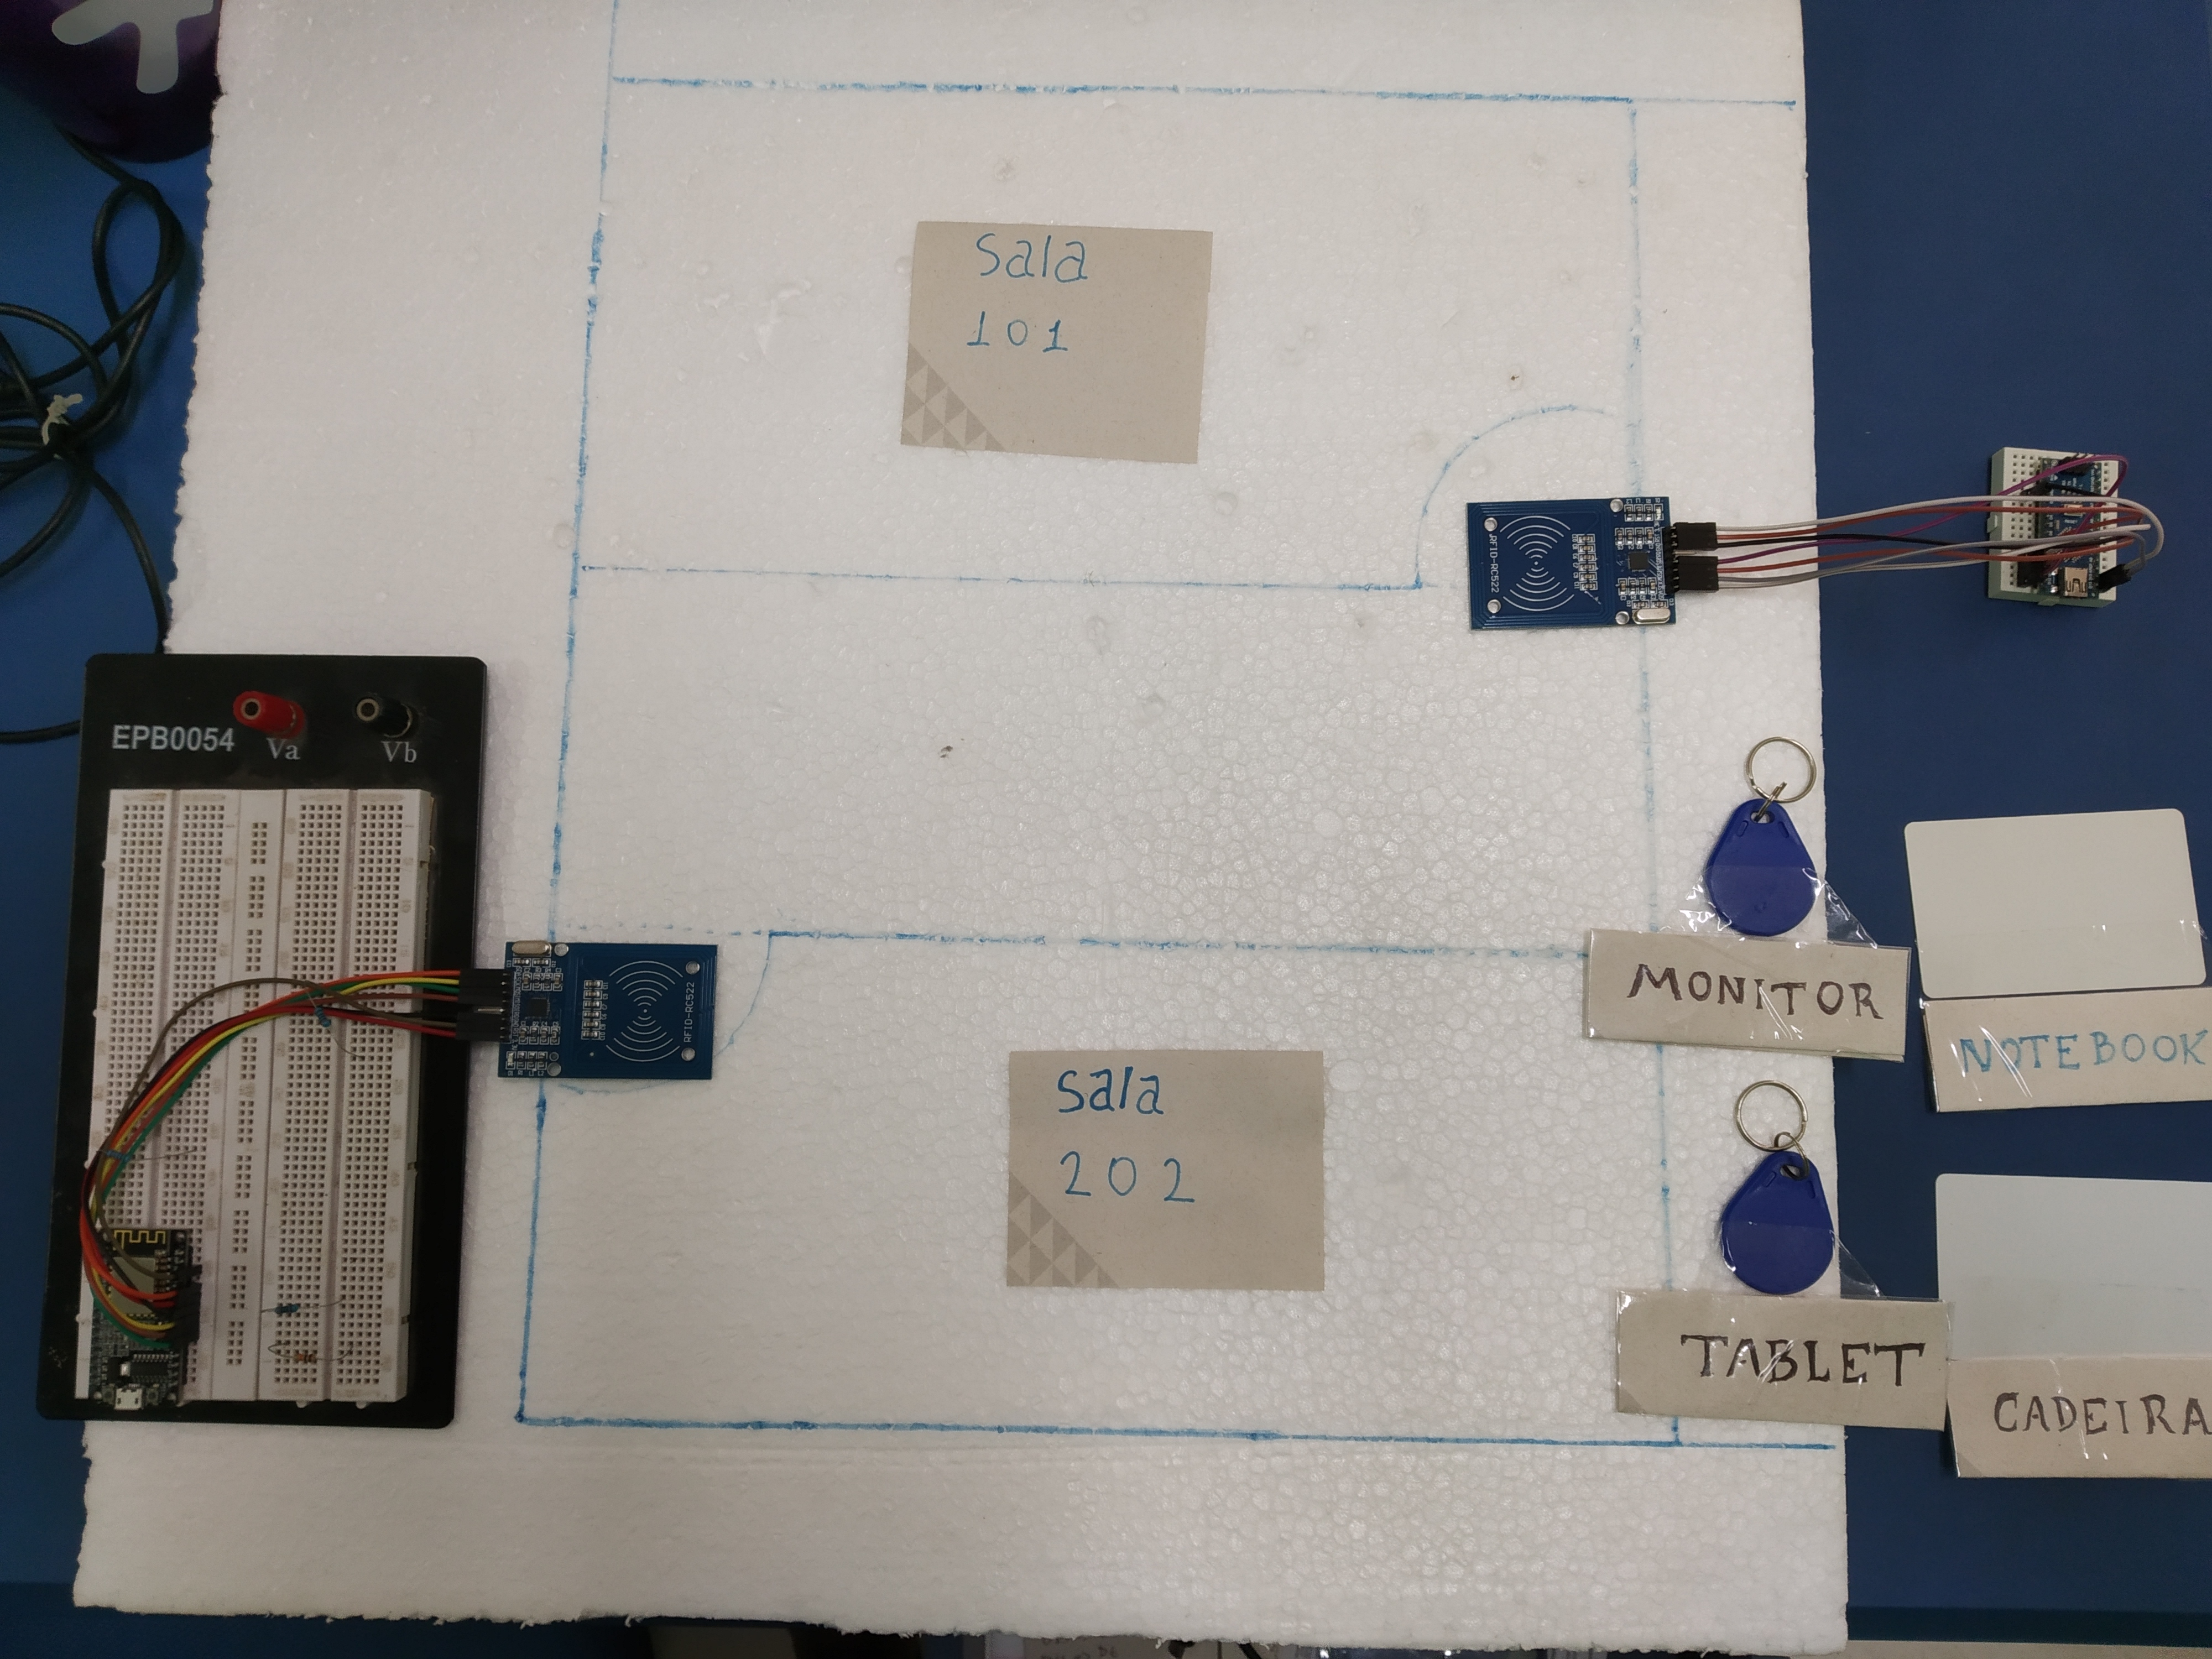
\includegraphics[width=1\textwidth]{Figuras/cenario.png}
              \legend{Fonte: Própria}
\end{figure}

\section{Execução dos experimentos e Análise dos Resultados}

Visando responder as questões de pesquisa no planejamento dos experimentos, o teste \textbf{(1)} no cenário do experimento foi executando  cadastrando as quatro etiquetas no sistema e identificando-as cada uma como um objeto diferente, duas etiquetas foram lidas pelo dispositivo de porta da sala $101$ e as outras duas foram lidas pelo dispositivo de porta da sala $202$, o \textit{pipiline} do processo pode ser visualizado na \autoref{fig:piptransicao} de \textbf{A} e \textbf{B}, esse processo de cadastro foi repetido por mais três vezes e o resultado final desse processo com as quatro etiquetas é apresentado no relatório do sistema INEXT na \autoref{fig:piptransicao} \textbf{C}.

\begin{figure}[ht]
        \centering\caption{Identificação dos objeto}
        \label{fig:piptransicao}
       \subfloat[A\label{fig:execution1a}]{
            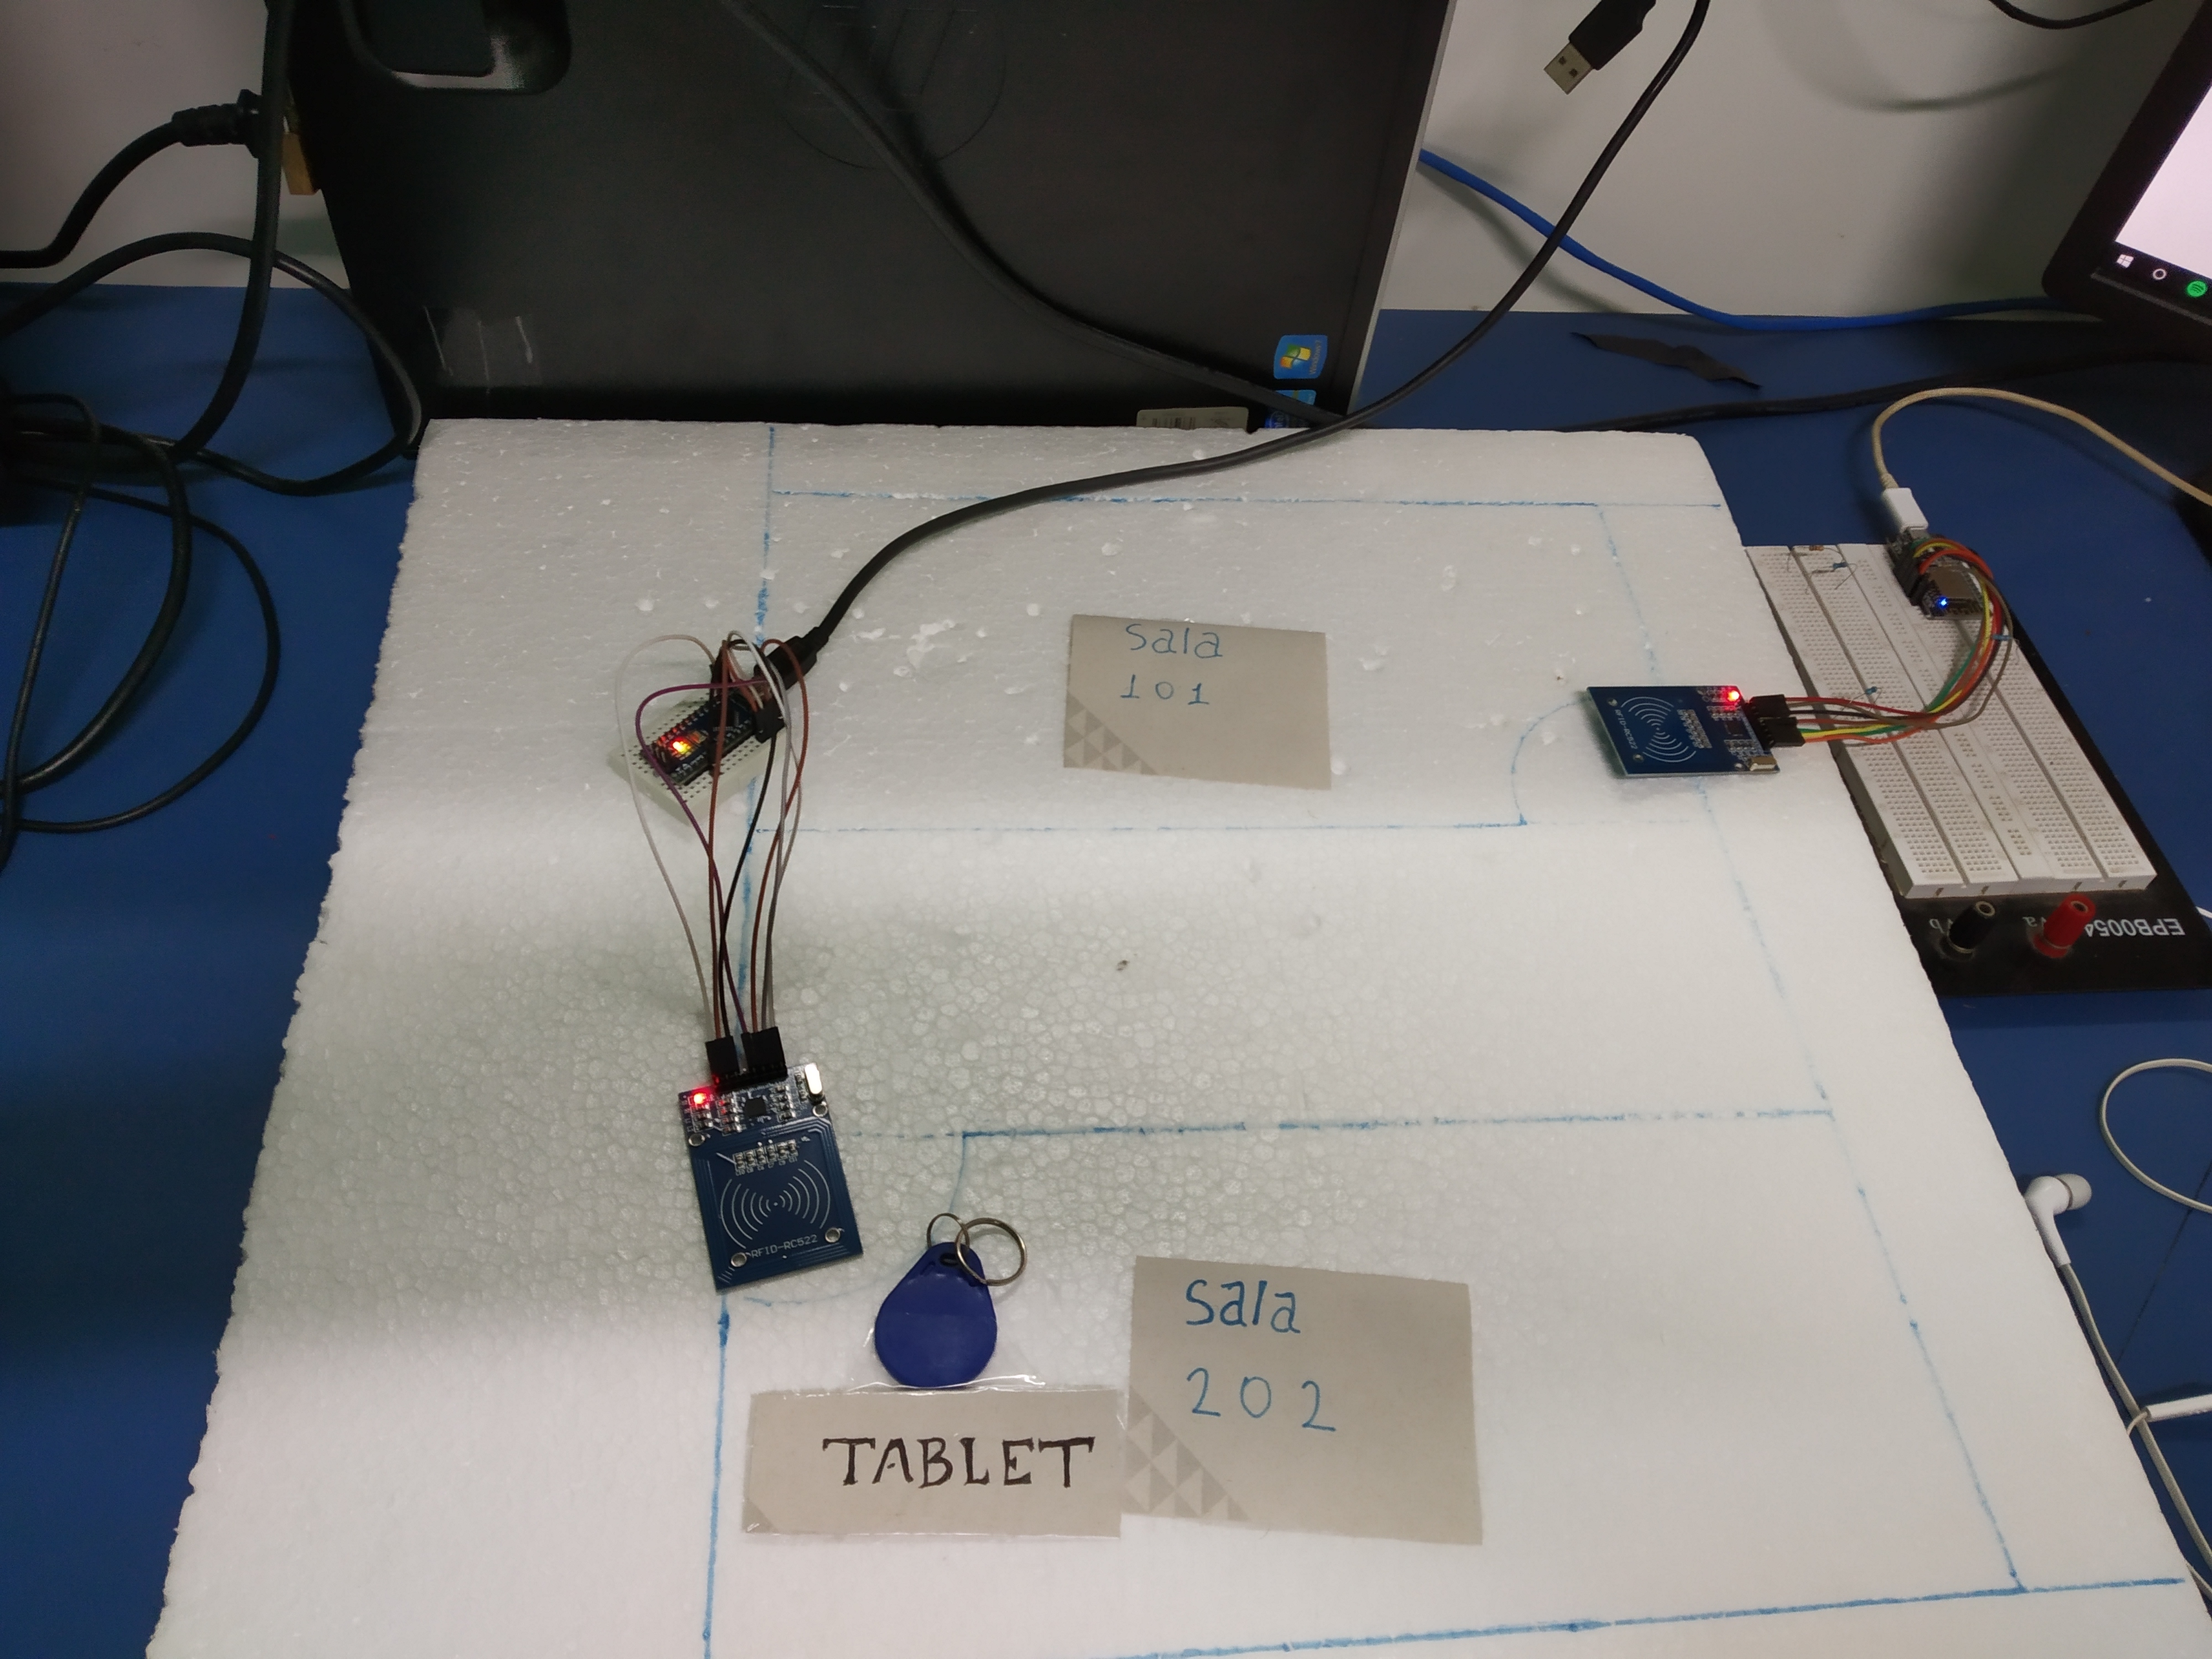
\includegraphics[width=0.5\textwidth]{Figuras/execucao1a.PNG}}
         \hspace{0.5cm}
%        \subfloat[B\label{fig:execution1b}]{
%             \includegraphics[width=0.7\textwidth]{Figuras/execucao1.PNG}}
%              \hspace{0.5cm}
\\
       \subfloat[B\label{fig:execution1c}]{
            \includegraphics[width=0.5\textwidth]{Figuras/execucao1br.PNG}}
        \hspace{0.5cm}
%        \subfloat[B\label{fig:execution1d}]{
%             \includegraphics[width=0.7\textwidth]{Figuras/execucao1c.PNG}}
%              \hspace{0.5cm}
\\
       \subfloat[C\label{fig:execution1f}]{
             \includegraphics[width=0.8\textwidth]{Figuras/execution1F.PNG}}
              \hspace{0.5cm}
      \legend{Fonte: Própria}
\end{figure}

% \par
\newpage
Ainda realização do teste \textbf{(1)} no cenário, o processo de transição dos objetos foi executado observando quando uma etiqueta é lida, quando sai da sala e quando entra na outra sala, esse \textit{pipiline} pode ser visto na \autoref{fig:piptransicaoTest11} de \textbf{A} até \textbf{C}. Foram executadas as transições para todos os objetos, onde a movimentação foi da sala $101$ para a sala $202$, e os da sala $202$ foram para a sala $101$.

\begin{figure}[ht]
        \centering\caption{Transição de objeto}
        \label{fig:piptransicaoTest11}
%        \subfloat[A\label{fig:execution2a}]{
%             \includegraphics[width=0.4\textwidth]{Figuras/execution2a.png}}
%          \hspace{0.5cm}
       \subfloat[A\label{fig:execution2b}]{
            \includegraphics[width=0.5\textwidth]{Figuras/execution2c.png}}
             \hspace{0.5cm}
             \\
       \subfloat[B\label{fig:execution2c}]{
            \includegraphics[width=0.7\textwidth]{Figuras/execution2b.png}}
        \hspace{0.7cm}
%        \subfloat[D\label{fig:execution2d}]{
%             \includegraphics[width=0.4\textwidth]{Figuras/execution2d.png}}
%              \hspace{0.5cm}
\\
       \subfloat[C\label{fig:execution2c}]{
             \includegraphics[width=0.7\textwidth]{Figuras/execution2e.png}}
              \hspace{0.5cm}
        
      \legend{Fonte: Própria}
\end{figure}

\newpage

% \par
No teste \textbf{(2)} do cenário experimental, foram criados dois usuário na tela de quem deve ser notificado a transição dos objetos para receber as notificações via e-mail. Para isso foi utilizado os e-mails do próprio autor deste trabalho, que utilizam os servidores de \textit{webmail} Gmail e Outlook, em seguida foi criado restrição para cada objeto monitorado no sistema. Na tela principal do sistema INEXT, cada objeto possui uma opção para editar ao seu lado, foi editado um objeto por vez colocando no campo restrição o mesmo nome que ele possuía no campo de \texttt{localização(sala)}. O cadastro dos usuários e a edição dos objetos pode ser visualizado no \textit{pipiline} da \autoref{fig:cadRest}.

\newpage

\begin{figure}[ht]
        \centering\caption{Cadastro de usuários e Criação de Restrições de objeto}
        \label{fig:cadRest}
%        \subfloat[A\label{fig:execution3a}]{
%             \includegraphics[width=0.4\textwidth]{Figuras/execution3a.png}}
%          \hspace{0.5cm}
       \subfloat[A\label{fig:execution3b}]{
            \includegraphics[width=0.7\textwidth]{Figuras/execution3b.png}}
             \hspace{0.5cm}
             \\
%        \subfloat[C\label{fig:execution3c}]{
%             \includegraphics[width=0.4\textwidth]{Figuras/execution3c.png}}
%         \hspace{0.5cm}
%        \subfloat[D\label{fig:execution3d}]{
%             \includegraphics[width=0.4\textwidth]{Figuras/execution3d.png}}
%              \hspace{0.5cm}
       \subfloat[B\label{fig:execution3e}]{
             \includegraphics[width=0.7\textwidth]{Figuras/execution3e.png}}
              \hspace{0.5cm}
      \legend{Fonte: Própria}
\end{figure}

\par
Ainda no teste \textbf{(2)} foi realizado processo de transição com os objetos, afim de verificar se o sistema notifica os usuários através do e-mail e na tela inicial quando o sistema proposto identifica que um dado objeto viola a sua restrição, ou seja, um dado objeto é identificado em uma sala para o qual não foi designado. A execução desta operação é apresentada na \autoref{fig:transicaoeRest}. Foram realizadas transições para todos os objetos com restrições.

\begin{figure}[ht]
        \centering\caption{Transições com Restrições}
        \label{fig:transicaoeRest}
%        \subfloat[A\label{fig:execution4a}]{
%             \includegraphics[width=0.4\textwidth]{Figuras/execution4a.png}}
%          \hspace{0.5cm}
%        \subfloat[B\label{fig:execution4b}]{
%             \includegraphics[width=0.4\textwidth]{Figuras/execution4b.png}}
%              \hspace{0.5cm}
       \subfloat[A\label{fig:execution4c}]{
            \includegraphics[width=0.5\textwidth]{Figuras/execution4c.png}}
        \hspace{0.5cm}        
        \\
       \subfloat[B\label{fig:execution4d}]{
            \includegraphics[width=0.5\textwidth]{Figuras/execution4d.png}}
             \hspace{0.5cm}
             \\
%        \subfloat[E\label{fig:execution4c}]{
%              \includegraphics[width=0.4\textwidth]{Figuras/execution4e.png}}
%               \hspace{0.5cm}
%         \subfloat[E\label{fig:execution4d}]{
%              \includegraphics[width=0.4\textwidth]{Figuras/execution4e.png}}
%               \hspace{0.5cm}      
        \subfloat[C\label{fig:execution4e}]{
             \includegraphics[width=0.7\textwidth]{Figuras/execution4e.png}}
              \hspace{0.5cm}
      \legend{Fonte: Própria}
\end{figure}

No teste \textbf{(3)} no cenário é executado o levantamento de todos os objetos monitorados (o inventário) pelo sistema INEXT em suas respectivas salas. Neste sentido, na tela web do sistema INEXT deve ser executado as seguintes ações: primeiramente é necessário ir até a tela \texttt{Ger. de Salas} para verificar as salas cadastradas no sistema e não há repetição de uma mesma sala; e em seguida ir para a tela \texttt{Inventário}, o inventário é gerado referente aquele momento, se ocorrer qualquer operação após a geração do inventário deverá ser realizado o processo novamente. O resultado da execução desse processo é apresentado na \autoref{fig:invent}.

% \todo[inline]{Sugiro adicionar um texto fazendo uma discussão sobre como é o inventário da UFRR atual e as vantagens que o sistema pode trazer}

% \begin{figure}[ht]
%         \centering\caption{Inventário}
%         \label{fig:invent}
% %        \subfloat[A\label{fig:execution5a}]{
% %             \includegraphics[width=0.4\textwidth]{Figuras/execution5a.png}}
% %          \hspace{0.5cm}
%        \subfloat[\label{fig:execution5b}]{
%             \includegraphics[width=0.4\textwidth]{Figuras/execution5b.png}}
%              \hspace{0.5cm}
% %        \subfloat[C\label{fig:execution5c}]{
% %             \includegraphics[width=0.4\textwidth]{Figuras/execution5c.png}}
% %         \hspace{0.5cm}
% %        \subfloat[D\label{fig:execution5d}]{
% %             \includegraphics[width=0.4\textwidth]{Figuras/execution5d.png}}
% %              \hspace{0.5cm}
% %        \subfloat[E\label{fig:execution5c}]{
% %              \includegraphics[width=0.4\textwidth]{Figuras/execution5e.png}}
% %               \hspace{0.5cm}
% %         
%       \legend{Fonte: Própria}
% \end{figure}

\begin{figure}[htb]
      \caption{\label{fig:invent}{Inventário}}
      \centering
      \includegraphics[width=0.8\textwidth]{Figuras/execution5d.png}
      \legend{Fonte: Própria}
\end{figure}

\subsection{Resultados}

Após a execução dos testes, foram obtidos os resultados apresentados na \autoref{tab:resultados}, onde cada linha representa: um cenário de execução com o seu respectivo número de execuções; número de execuções em que o sistema INEXT funcionou de maneira correta (\textbf{Funcionou}); números de execuções em que o sistema INEXT por alguma questão não funcionou perfeitamente (\textbf{Parcialmente}); e o número de execuções em que o sistema falhou durante a suas execução, ou seja, não retornou o resultado esperado (\textbf{Falhou}).

%\todo[inline]{O ideal é que o número de execuções seja entre 7 ou 13 vezes}

\begin{table}[ht]
  \centering
  \caption{Resultados}
  \label{tab:resultados}
  \begin{tabular}{|c|c|c|c|c|c|}
     \hline
    & \textbf{N$^{\circ}$ de execuções} & \textbf{Funcionou} & \textbf{Parcialmente} & \textbf{Falhou} \\
    \hline
    Teste 1 & 8 & 7 & - & 1\\
    \hline
    Teste 2 & 8 & 8 & - & -\\
    \hline
    Teste 3 & 7 & 6 & 1 & -\\
    \hline

  \end{tabular}
\end{table}

\par
O INEXT conseguiu localizar objetos rastreados por RFID em ambientes confinados, porém o sistema não proporciona a posição especifica do objeto no ambiente, exemplo, no lado direito da sala. O sistema também foi capaz de identificar os objetos, mas essa etapa ainda ocorre de maneira manual necessitando ser realizada por usuários a edição dos objeto no sistema após ter o seu cadastro no sistema. %\todo[color=green]{Não está claro isso, parece que alguem tem ir na sala para ver o objeto}.
Durante os teste houve uma execução em que os script em Python que é responsável por ler os dados da porta serial do Arduíno Nano, gerar um JSON e enviar para o servidor via POST, %\todo[color=green]{responsável por?}
travou e não enviou os JSON's gerados para o servidor devido ao cabo USB que foi tocado no momento e se desconectou, sendo necessário parar o script e iniciar novamente e assim realizar a leitura novamente para que a etiqueta tivesse a localização correta.%e ocasionando a perda da localização de um objeto\todo{Por qual razão o script travou, justificar e descrever como melhorar isso.}.

\par
O sistema proporcionou uma boa forma de gerenciar os objetos, de acordo com os resultados do experimento. De forma que por meio do uso do sistema INEXT foi possível informar os usuários sobre as violação de restrições através do e-mail e também na tela principal do sistema. 
% Assim, gerando uma nova tabela com os objetos que violaram suas restrições.
% 
% \par
Durante a primeira tentativa de gerar o inventário dos objetos cadastrados no sistema, houve repetição de dados justamente porque foram criadas salas repetidas no banco de dados, esse problema pode ser solucionado acessando a tela \texttt{Ger. de Salas} e remover as salas repetidas, dessa forma a geração do inventário funcionou sem a repetição dos objetos e salas. %\todo[color=green]{Descrever como evitar isso dentro do INEXT}
\par
Afim de ter uma melhor avaliação do sistema foi elaborada um questionário contendo quatro questões, e aplicado a três pessoas que foram/são coordenadores/chefes de departamentos de cursos da UFRR. As as questões são listadas abaixo:
\begin{enumerate}
    \item De 0 à 10, você acha que o sistema pode auxiliar o gerenciamento dos bens da universidade?
    \item De 0 à 10, qual nota você daria para avaliar essa solução aplicada ao problema?
    \item De 0 à 10, qual a probabilidade de indicar o sistema para os funcionários da UFRR que realizam a tarefa de gerenciamento e levantamento de patrimônio?
   % \item Quais melhorias você sugere?
\end{enumerate}

\par
As perguntas 1, 2 e 3 possuem representatividade quantitativa em que: 0 e 1 são muito ruim, 2 e 3 ruim, 5 e 6 razoável, 7 e 8 bom, 9 e 10 muito bom. % A questão de número quatro é subjetiva possibilitando que cada pessoa contribua com possíveis melhorias.
O resultado do questionário pode ser visto na \autoref{tab:questionario}.
\begin{table}[ht]
\centering
\caption{Dados coletados do questionário realizado}
\begin{tabular}{c|c|c|c||c|}
\cline{2-5}
                                          & \textbf{Pessoa 1} & \textbf{Pessoa 2} & \textbf{Pessoa 3} & \textbf{Média} \\ \hline
\multicolumn{1}{|c|}{\textbf{Pergunta 1}} & 10                & 9                 & 10                & 9.66           \\ \hline
\multicolumn{1}{|c|}{\textbf{Pergunta 2}} & 8                 & 8                 & 7                 & 7.66           \\ \hline
\multicolumn{1}{|c|}{\textbf{Pergunta 3}} & 9                 & 9                 & 10                & 9.33           \\ \hline
\end{tabular}
\label{tab:questionario}
\end{table}
\par
A média das respostas em relação a pergunta 1 é de 9.66, mostrando que o sistema pode auxiliar o gerenciamento e levantamento de bens da universidade, de forma que se implantando proporciona facilidade em relação como a maneira que o levantamento é realizado atualmente, em que é necessário a visita de um funcionário em todas as salas verificando-as e anotando todos as referencias dos objetos lá situados.

\par
Na pergunta de número 2, as respostas obtiveram média igual a 7.66, o que mostra que os sistema é bom, porém o sistema não é capaz de resolver todos os problemas, por exemplo, quando o objeto está em transição, se por algum motivo não entrar em uma outra sala o objeto não possuirá localização no sistema. Por fim, a pergunta número 3, obteve média igual 9.33, que de modo geral mostra que o sistema possui grande potencial de aplicabilidade e grandes indícios que pode ser indicada para os funcionários da UFRR que executam essa função.

